\documentclass{article}
\usepackage{fullpage}
\usepackage{caption}
\usepackage{subcaption}
\usepackage{amsmath}
\usepackage{commath}
\usepackage{graphicx}
\usepackage{listings}
\usepackage{tgbonum}
\usepackage{xcolor}
\usepackage{booktabs}
\lstset{
language=Python,
basicstyle=\footnotesize\rmfamily,
numbers=left,
basicstyle=\small,
tabsize=1,
frame=single,
keywordstyle=\color{blue},
xleftmargin=2em}
\begin{document}

\begin{center}
{\Large Numpy code for calculation multi-component adsorption isotherms using ideal adsorbed solution theory}
\end{center}
\section{Computer code}

Multicomponent adsorption isotherms are frequently predicted from single component isotherms using the well-known ideal adsorbed solution theory (IAST) introduced by Myers and Prausnitz.\cite{Myers1965} The advantage of IAST is also that it is able to compute mixture adsorption using any molar composition. Here, we consider a binary mixture only.

IAST is based on three assumptions: (1) all adsorbates have access to the same surface area of the sorbent, (2) the sorbent is inert, and (3) the mixture in the adsorbed phase behaves as an ideal solution at constant temperature and spreading pressure.

The spreading pressure $\pi$ can be thought of as the negative of the surface tension and can be calculated via the Gibbs isotherm\cite{Myers1965}
%
\begin{equation}
        \frac{{\pi}A}{RT} = \int_0^{P_i^0}\frac{q_i}{P} {\dif P}
	\label{eq:spreading_pressure}
\end{equation}
%
with $A$ the surface area of the sorbent, $R$ the gas constant, $T$ the temperature, $P_i^0$ the partial pressure for component $i$ at the spreading pressure, $q_i$ the single component $i$ adsorption isotherm and and $P_i$ the component pressure of the bulk phase. Here, $q_i$ is fitted to a Langmuir isotherm $q_i = q_\text{sat,i}b_iP/(1+b_iP)$. Integrating equation (\ref{eq:spreading_pressure}) analytically gives
%
\begin{equation}
	\int_0^{P_i^0}\frac{q_i}{P} {\dif P} =  q_\text{sat,i}\ln\Big({1+b_iP_i^0}\Big). 
\end{equation}
%
At equilibrium, the spreading pressures of all components are equivalent. Therefore, for a two-component system the following relation holds 
%
\begin{equation} 
	q_\text{sat,1}\ln{\Big(1+b_1\frac{Py_1}{x_1}\Big)} - q_\text{sat,2}\ln{\Big(1+b_2\frac{Py_2}{1-x_1}\Big)} = 0
	\label{eq:find_root}
\end{equation} 
%
with $x_2 = 1 - x_1$ and the adsorbed-vapour phase is described by an analog of Raoult's law 
%
\begin{equation}
        \frac{Py_i}{x_i} = P_i^0
\end{equation}
%
with $x_i$ being the mole fraction of component $i$ in the adsorbed phase. Listing 1 shows a routine that solves  equation (\ref{eq:find_root}) for $x_1$.

\begin{lstlisting}[caption={Find root of equation (\ref{eq:find_root}) and obtain $x_1$.}]
def iast_langmuir_analytical(x,data):
  P,y,isotherm = data[0],data[1],data[2]
  isotherm1 = isotherm[0]
  isotherm2 = isotherm[1]

  f = isotherm1[0]*np.log(1+isotherm1[1]*y[0]*P/x)-\
  isotherm2[0]*np.log(1+isotherm2[1]*((y[1]*P)/(1-x)))
  return f

f = fsolve(iast_langmuir_analytical,x0,args=data)
x[0] = f
x[1] = 1 - x[0]
\end{lstlisting}

The scipy function fsolve() returns the root of the function iast\_langmuir\_analytical(). This root is $x_1$ and for a two-component mixture $x_2 = 1 - x_1$. Next, the total adsorption capacity $q_T$ is obtained from
%
\begin{equation}
        \frac{1}{q_T} = \sum_{i}^N\frac{x_i}{q_i(P_i^0)}
	\label{eq:total_adsorbed_loading}
\end{equation}
%
with $q_i={x_i}q_T$. Here, $q_i$ (not $q_i(P_i^0$) is the actual adsorbed amount of component $i$ in the mixture. In the code, it is given as follows: 
%
\begin{lstlisting}[caption={Compute the mixture adsorption isotherms based on equation (\ref{eq:total_adsorbed_loading}).}]
q = langmuir(P*(S.y/x),S.params)

qtot = 1.0/np.sum(x/q)
q_mix = qtot * x
\end{lstlisting}
%
Remember that the variables $x$ and $S.y$ are numpy arrays!

\section{Example: equimolar methane/ethane mixture in ZIF-8 at 433 K.}
In the directory 'adsorption\_isotherms', you will find the input files and results of this section.

Figure \ref{fig:single_component_isotherms} show the (a) single and (b) multi component adsorption isotherm of methane and ethane in ZIF-8 at 433 K. These isotherms are calculated using grand-canonical Monte Carlo (GCMC) simulations using the RASPA-2.0 package.\cite{Dubbeldam2013} In the next subsection the simulations details are given. For more details on calculating adsorption properties using GCMC simulations the reader is refered to \cite{Frenkel2001,Dubbeldam2013,Dubbeldam2015} The Langmuir isotherm parameters are presented in Table \ref{tab:isotherm_parameters}.

\begin{figure}[h!]
\centering
\begin{subfigure}[h]{0.5\textwidth}
\centering
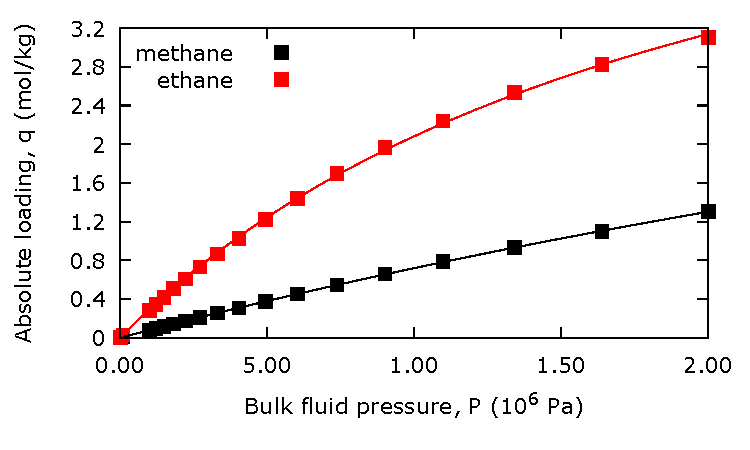
\includegraphics[width=1.0\textwidth]{./../adsorption_isotherms/singlecomponent_zif_methane_ethane_433K.pdf}
\subcaption{}
\end{subfigure}~
\begin{subfigure}[h]{0.5\textwidth}
\centering
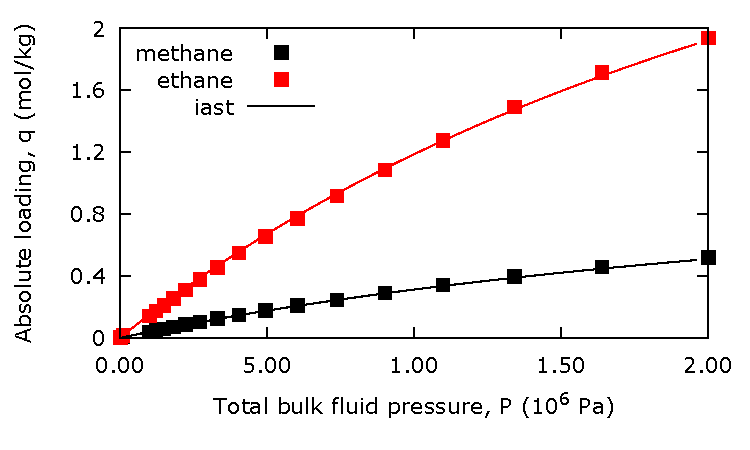
\includegraphics[width=1.0\textwidth]{./../adsorption_isotherms/multicomponent_zif_methane_ethane_433K.pdf}
\subcaption{}
\end{subfigure}
\caption{Adsorption isotherm of methane (black) and ethane (red) in ZIF-8 at 433 K. Data points are obtained from GCMC simulations. (a) Single component isotherm; solid lines are fitted Langmuir isotherms. (b) Multi component isotherms; solid lines are IAST predictions.}
\label{fig:single_component_isotherms}
\end{figure}

\clearpage

\subsection{Simulations details} 
The Van der Waals cut-off radius was set to 12.0 \AA. To maintain the minimum image convention, a 2 x 2 x 2 unit cell was used with a lattice constant of $a$ = 16.991 \AA. Non-bonding interactions are described using the Lennard-Jones potentials. For the framework, these are based on the DREIDING and UFF force field (GenericMOFs in RASPA-2.0) and for the adsorbates, the TraPPE force field is used. Note that the TraPPE force field is neutral, therefore no electrostatics are considered. The number of production cycles was set to 100000 and the number of initialization cycles to 50000. These are fairly standard settings but are sufficient for this system.  


\begin{table}[h!]
\centering
\caption{Langmuir isotherm parameters of methane and ethane.}
\label{tab:isotherm_parameters}
\begin{tabular}{l l l l}
\toprule
\multicolumn{2}{c}{methane} & \multicolumn{2}{c}{ethane}\\
$q_\text{sat,1}$ (mol/kg) & $b_1$ $\cdot$ 10$^{-7}$ (Pa$^{-1}$) & $q_\text{sat,2}$ (mol/kg) & $b_2$  $\cdot$ 10$^{-7}$ (Pa$^{-1}$) \\
\midrule
6.85 & 1.18 & 6.37 & 4.85 \\
\bottomrule
\end{tabular}
\end{table}




\bibliographystyle{unsrt}
\bibliography{references}

\end{document}
